\section{Experimental protocol}
\label{app:experimental-protocol}

\paragraph{Training data and selected fits.}
Table~\ref{tab:main} gives the DFlash fit time for each selected target and Table~\ref{tab:eagle} gives the corresponding EAGLE-3 time. All selected fits use two L40S GPUs and a global batch of eight. For Qwen3-4B LoRA-fine-tuned targets, DFlash trains five identity-initialized maps on 4{,}096 saved, target-generated responses from the task domain. It samples 32 valid response anchors per example, trains AUF for one epoch and uses a peak learning rate of $10^{-4}$. Qwen3-8B LoRA-fine-tuned targets use the same 4{,}096-response, 32-anchor, one-epoch AUF recipe and learning rate. Each response is capped at 4{,}096 tokens during generation, and each anchor has at most 15 supervised proposal positions.

For DFlash cross-transfer, each selected fit trains five Xavier-initialized maps on 16{,}384 NuminaMath-derived trajectories with target-generated responses capped at 4{,}096 tokens~\citep{li2024numinamath}. The original and new targets process the same saved token sequences. Reconstruction supervises 25\% of prompt positions and a separate 25\% of response positions. It trains for three epochs with peak learning rate $10^{-3}$. Each cross-transfer fit is shared across its four evaluation workloads, so its optimizer-loop time is reported once per target--drafter pair in Tables~\ref{tab:main} and~\ref{tab:eagle}, not once per dataset. EAGLE-3 uses the same selected cross-transfer data, position sampling, epoch count, and learning rate, but trains three maps. For LoRA-fine-tuned targets, EAGLE-3 trains three identity-initialized maps with AUF on 4{,}096 saved responses, up to 32 response anchors per example, one epoch, and peak learning rate $10^{-4}$. Ablations in Section~\ref{sec:ablations} use their stated data sizes, supervision coverage, and objectives rather than these selected recipes.

For the scaling experiments, counts denote training presentations. When a source dataset contains fewer than 4{,}096 available examples, examples are repeated to reach the required count.

\paragraph{Single-request evaluation.}
The DFlash measurements in Tables~\ref{tab:main} and~\ref{tab:llama-transfer} use BF16 Transformers inference with greedy decoding and one serial request per L40S GPU~\citep{wolf2020transformers}. Each workload has 128 fixed prompts. Generation stops at the natural end-of-sequence token or a 2{,}048-token response cap, except KiCad, which uses an 8{,}192-token cap. Thinking is disabled for Qwen3. Throughput is the arithmetic mean of each request's returned-token count divided by its elapsed generation time. Autoregressive, reference-drafter, and mapped-drafter measurements use the same prompt cohort and decoding contract. Acceptance length is the pooled emitted-token count divided by verification steps and includes the target's correction contribution. EAGLE-3 uses its own pinned tree settings and emitted-token counters, so its acceptance lengths are not numerically interchangeable with DFlash's.

\paragraph{Concurrent serving.}
Serving runs use vLLM 0.28.0, BF16, greedy decoding, and fixed prompts~\citep{kwon2023vllm}. Cross-transfer serving uses one L40S per engine, 128 prompts per workload, a 2{,}048-token response cap, and 16 concurrent clients for Table~\ref{tab:transfer-serving}. The Qwen3-8B transfer additionally measures 1, 8, and 32 clients. The LoRA-fine-tuned shared-serving experiment in Figure~\ref{fig:serving} sends a fixed mixture of 384 requests, 128 for each of three task adapters. Its response cap is 2{,}048 tokens for GSM8K and NanoCoder and 8{,}192 for KiCad. Serving throughput divides all returned tokens by workload wall time, including drain, rather than averaging per-request rates. Native, mapped, and autoregressive runs receive the same inputs.

\subsection{Architecture and objective ablations}
\label{app:architecture-objective}

The placement comparison uses LoRA-fine-tuned Qwen3-4B targets and the same token-supervision setting for every row. The objective comparison uses identity-initialized maps for LoRA-fine-tuned targets and Xavier-initialized maps for Qwen3-8B $\leftarrow$ Qwen3-4B cross-transfer. Its cross-transfer rows use 8{,}192 examples, so they are separate recipe comparisons from the selected 16{,}384-example result in Table~\ref{tab:main}.

\begin{table}[htbp]
\centering
\caption{Placement ablation on LoRA-fine-tuned Qwen3-4B targets. Throughput gains are percentages over the unadapted drafter. HM is the harmonic mean of workload ratios. Best in each result column is bold and second best is underlined.}
\label{tab:ablation-placement}
\small
\setlength{\tabcolsep}{4.3pt}
\begin{tabular}{lrrrrr}
\toprule
Trained object & Parameters & GSM8K (\%) & KiCad (\%) & NanoCoder (\%) & HM \\
\midrule
Five per-stream maps (RelaySpec) & 32.8M & $\mathbf{+37.6}$ & $\mathbf{+89.5}$ & $+8.1$ & $\mathbf{1.376}\times$ \\
Single fused projection & 32.8M & $+32.4$ & $+44.5$ & $\underline{+8.2}$ & $1.265\times$ \\
Draft-transformer LoRA, rank 128 & 36.7M & $\underline{+36.4}$ & $+75.5$ & $\mathbf{+9.8}$ & $\underline{1.355}\times$ \\
Single joint map over all streams & 163.8M & $+24.3$ & $\underline{+88.4}$ & $-7.0$ & $1.244\times$ \\
Rank-128 maps & 3.3M & $+3.2$ & $+58.4$ & $-28.8$ & $0.999\times$ \\
Rank-56 maps & 1.4M & $-21.9$ & $+35.1$ & $-49.3$ & $0.751\times$ \\
Rank-28 maps & 0.7M & $-43.1$ & $+12.8$ & $-62.5$ & $0.565\times$ \\
\bottomrule
\end{tabular}
\end{table}

\subsection{Scaling fit times}
\label{app:scaling-fit-times}

\begin{figure}[htbp]
\centering
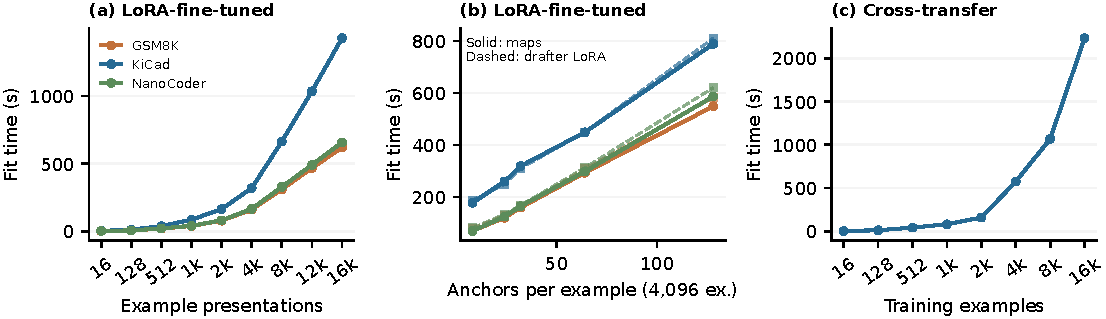
\includegraphics[width=\linewidth]{figures/relayspec_scaling_fit_times.pdf}
\caption{Fit times for the scaling measurements in Figure~\ref{fig:scaling}.}
\end{figure}

\begin{table}[htbp]
\centering
\caption{Training recipes on LoRA-fine-tuned targets (top, relative to unadapted) and Qwen3-8B $\leftarrow$ Qwen3-4B (bottom, relative to native). Entries are throughput ratios. MSE50 and MSE100 use 50\% and 100\% of positions. Best in each setting and column is bold and second best is underlined.}
\label{tab:ablation-objective}
\small
\setlength{\tabcolsep}{4pt}
\begin{tabular}{llrrrrr}
\toprule
Setting & Objective & \multicolumn{4}{c}{Workload} & HM \\
\midrule
 & & GSM8K & KiCad & NanoCoder & & \\
\cmidrule(lr){3-5}
LoRA-fine-tuned & Accept-until-fail & $\mathbf{1.376}\times$ & $\underline{1.895}\times$ & $\mathbf{1.081}\times$ & & $\mathbf{1.376}\times$ \\
 & Decaying cross-entropy & $\underline{1.368}\times$ & $\mathbf{1.935}\times$ & $\underline{1.031}\times$ & & $\underline{1.353}\times$ \\
 & Reconstruction, MSE50 & $1.011\times$ & $1.191\times$ & $0.977\times$ & & $1.052\times$ \\
\midrule
 & & Math & GSM8K & Code & Chat & \\
\cmidrule(lr){3-6}
Cross-transfer & Reconstruction, MSE100 & $\underline{0.998}\times$ & $\mathbf{0.990}\times$ & $\underline{0.828}\times$ & $\mathbf{0.891}\times$ & $\mathbf{0.921}\times$ \\
 & Reconstruction, MSE50 & $\mathbf{0.999}\times$ & $\underline{0.975}\times$ & $\mathbf{0.832}\times$ & $\underline{0.888}\times$ & $\underline{0.919}\times$ \\
 & Decaying cross-entropy & $0.886\times$ & $0.919\times$ & $0.406\times$ & $0.573\times$ & $0.623\times$ \\
 & Accept-until-fail & $0.884\times$ & $0.911\times$ & $0.385\times$ & $0.558\times$ & $0.604\times$ \\
\bottomrule
\end{tabular}
\end{table}

\begin{table}[htbp]
\centering
\caption{Linear maps and nonlinear branches on matched training data. Throughput is in tokens/s. Best of each pair is bold and second best is underlined.}
\label{tab:ablation-capacity}
\small
\begin{tabular}{llrrrrr}
\toprule
& & \multicolumn{2}{c}{Tokens/s} & & \multicolumn{2}{c}{$\tau$} \\
\cmidrule(lr){3-4}\cmidrule(lr){6-7}
Setting & Workload & Linear & Nonlinear & Change & Linear & Nonlinear \\
\midrule
LoRA-fine-tuned & GSM8K & \textbf{179.83} & \underline{177.94} & $-1.05\%$ & \textbf{5.988} & \underline{5.953} \\
 & KiCad & \underline{312.47} & \textbf{321.76} & $+2.97\%$ & \underline{11.256} & \textbf{11.411} \\
 & NanoCoder & \textbf{171.73} & \underline{169.74} & $-1.16\%$ & \textbf{5.552} & \underline{5.520} \\
\midrule
Cross-transfer & Math & \textbf{220.26} & \underline{215.71} & $-2.07\%$ & \textbf{7.984} & \underline{7.980} \\
 & GSM8K & \textbf{176.87} & \underline{174.56} & $-1.31\%$ & \underline{6.242} & \textbf{6.257} \\
 & Code & \underline{127.61} & \textbf{128.41} & $+0.63\%$ & \underline{4.739} & \textbf{4.782} \\
 & Chat & \textbf{80.93} & \underline{80.78} & $-0.20\%$ & \underline{2.887} & \textbf{2.902} \\
\bottomrule
\end{tabular}
\end{table}

\subsection{Concurrent serving details}
\label{app:serving-details}

Table~\ref{tab:lora-serving-16} gives the 16-client point from Figure~\ref{fig:serving}. It serves a fixed, equal mixture of the three LoRA-fine-tuned targets. The following subsections give the separate multi-LoRA router and pooled-map experiments. Table~\ref{tab:transfer-serving} gives all measured cross-transfer pairs at 16 clients. The Qwen3-8B $\leftarrow$ Qwen3-4B pair is also shown across client counts in Figure~\ref{fig:transfer-serving}.

\begin{table}[htbp]
\centering
\caption{LoRA-fine-tuned shared serving at 16 concurrent clients. The fixed mixture contains 384 requests, with 128 requests per target. Aggregate and mean per-request throughput are measured in tokens/s.}
\label{tab:lora-serving-16}
\small
\begin{tabular}{lrrr}
\toprule
Mode & Aggregate throughput & Mean per-request throughput & $\tau$ \\
\midrule
Autoregressive & 595.46 & 40.91 & -- \\
Unadapted drafter & 2097.75 & 124.67 & 5.832 \\
RelaySpec & 3693.09 & 175.93 & 10.496 \\
\bottomrule
\end{tabular}
\end{table}

\subsubsection{Multiple LoRAs and a learned router}

The multi-LoRA experiment uses one BF16 Qwen3-4B target backbone, one frozen DFlash drafter, and the GSM8K, KiCad, and NanoCoder target LoRAs.  Each LoRA has a separate fusion-rank-56 AUF map bank.  Each bank is trained on 4{,}096 unique examples from its domain, with a 4{,}096-response-token cap, eight sampled anchors per response, 15 proposal labels per anchor, and 2{,}000 optimizer updates.  The maps use random-$A$/zero-$B$ initialization, AdamW at $10^{-4}$, 100 warmup steps followed by cosine decay, and global batch size 8 on two L40S GPUs.  The target, drafter transformer, normalization layers, embeddings, and output head remain frozen.  The three fits take 3.83, 10.51, and 4.54 minutes for GSM8K, KiCad, and NanoCoder, respectively.

In the explicit-ID condition, the request specifies which target LoRA is active and selects its matching map bank.  For the learned condition, a frozen prompt-only hard router selects one pair before generation.  It is a multinomial logistic-regression classifier over word unigram and bigram TF--IDF features.  The router trains on 4{,}096 user prompts per domain with 32{,}768 maximum features, $C=1$, and L-BFGS.  It fits in 0.944 CPU seconds and reaches 99.740\% held-out source-domain accuracy.  The selected pair remains fixed throughout a response.  It is therefore a hard request-level mixture of LoRA/map experts, rather than a token-level mixture.

\begin{table}[htbp]
\centering
\caption{Complete 12-client multi-LoRA map-bank results. Each repeat serves 384 requests, with 128 requests per target LoRA. Speedup is relative to the unadapted drafter.}
\label{tab:lora-router}
\small
\begin{tabular}{lrrr}
\toprule
Selection & Repeat & Speedup & $\tau$ \\
\midrule
Explicit target ID & 0 & 1.3176$\times$ & 7.678 \\
Explicit target ID & 1 & 1.3288$\times$ & 7.678 \\
Learned hard router & 0 & 1.3212$\times$ & 7.680 \\
Learned hard router & 1 & 1.3243$\times$ & 7.680 \\
\bottomrule
\end{tabular}
\end{table}

\subsubsection{One pooled map across the three LoRAs}

We also train one fusion-rank-56 AUF map bank on the union of the three domains.  It uses the same per-domain examples, response cap, anchors, labels, initialization, and optimizer settings as the separate banks.  Domain-homogeneous batches alternate round robin.  Each domain receives 2{,}000 updates, so the shared optimizer runs for 6{,}000 updates and sees 48{,}000 response presentations.  The pooled fit takes 27.12 minutes on two L40S GPUs.  Table~\ref{tab:lora-pooled} gives all measurements under explicit target IDs and the learned router.  The autoregressive and separate-bank controls were inherited without rerunning from the corresponding matched serving measurements.

\begin{table*}[htbp]
\centering
\caption{Complete 12-client pooled-map results for the three-LoRA mixture. Aggregate throughput is measured in tokens/s. Fit time is measured in minutes on two L40S GPUs. A dash denotes a configuration with no mapper fit.}
\label{tab:lora-pooled}
\small
\resizebox{\textwidth}{!}{%
\begin{tabular}{lllr rrr}
\toprule
Selection & Repeat & Configuration & Aggregate throughput (tokens/s) & $\tau$ & Speedup vs. autoregressive & Fit time (min) \\
\midrule
Explicit target ID & 0 & Autoregressive & 195.39 & -- & 1.0000$\times$ & -- \\
 & 0 & Unadapted drafter & 1273.98 & 5.8553 & 6.5200$\times$ & -- \\
 & 0 & Three map banks & 1678.61 & 7.6782 & 8.5909$\times$ & 3.83 / 10.51 / 4.54 \\
 & 0 & One pooled map & 1671.89 & 7.6170 & 8.5565$\times$ & 27.12 \\
 & 1 & Autoregressive & 194.40 & -- & 1.0000$\times$ & -- \\
 & 1 & Unadapted drafter & 1273.32 & 5.8553 & 6.5500$\times$ & -- \\
 & 1 & Three map banks & 1691.96 & 7.6782 & 8.7036$\times$ & 3.83 / 10.51 / 4.54 \\
 & 1 & One pooled map & 1673.98 & 7.6170 & 8.6111$\times$ & 27.12 \\
\midrule
Learned hard router & 0 & Autoregressive & 195.45 & -- & 1.0000$\times$ & -- \\
 & 0 & Unadapted drafter & 1280.52 & 5.8560 & 6.5518$\times$ & -- \\
 & 0 & Three map banks & 1691.87 & 7.6798 & 8.6565$\times$ & 3.83 / 10.51 / 4.54 \\
 & 0 & One pooled map & 1682.03 & 7.6188 & 8.6061$\times$ & 27.12 \\
 & 1 & Autoregressive & 195.59 & -- & 1.0000$\times$ & -- \\
 & 1 & Unadapted drafter & 1285.61 & 5.8560 & 6.5729$\times$ & -- \\
 & 1 & Three map banks & 1702.59 & 7.6798 & 8.7048$\times$ & 3.83 / 10.51 / 4.54 \\
 & 1 & One pooled map & 1695.52 & 7.6188 & 8.6687$\times$ & 27.12 \\
\bottomrule
\end{tabular}
}
\end{table*}

\begin{table}[htbp]
\centering
\caption{Cross-transfer serving at 16 concurrent clients. Aggregate throughput is measured in tokens/s. The higher throughput is bold and the lower is underlined.}
\label{tab:transfer-serving}
\small
\begin{tabular}{llrrr}
\toprule
Target $\leftarrow$ drafter & Workload & Native (tokens/s) & RelaySpec (tokens/s) & RelaySpec/native \\
\midrule
Qwen3-8B $\leftarrow$ Qwen3-4B & Math & \underline{2524.31} & \textbf{2716.26} & 1.076$\times$ \\
 & GSM8K & \underline{2207.43} & \textbf{2262.03} & 1.025$\times$ \\
 & Code & \textbf{1748.19} & \underline{1548.47} & 0.886$\times$ \\
 & Chat & \textbf{1091.14} & \underline{1065.93} & 0.977$\times$ \\
\midrule
Qwen3-4B $\leftarrow$ Qwen3-8B & Math & \textbf{4482.42} & \underline{3710.76} & 0.828$\times$ \\
 & GSM8K & \textbf{3160.99} & \underline{3078.87} & 0.974$\times$ \\
 & Code & \textbf{2840.15} & \underline{2002.79} & 0.705$\times$ \\
 & Chat & \textbf{1888.69} & \underline{1431.21} & 0.758$\times$ \\
\midrule
Llama3.1-8B $\leftarrow$ Qwen3-4B & Math & \textbf{1894.99} & \underline{1046.94} & 0.553$\times$ \\
 & GSM8K & \textbf{1354.50} & \underline{853.13} & 0.630$\times$ \\
 & Code & \textbf{1296.83} & \underline{636.97} & 0.491$\times$ \\
 & Chat & \textbf{1440.04} & \underline{524.40} & 0.364$\times$ \\
\bottomrule
\end{tabular}
\end{table}

\section{Complete analysis probe results}
\label{app:analysis-probes}

\makeatletter
\setlength{\@fptop}{0pt}
\setlength{\@fpsep}{12pt}
\setlength{\@fpbot}{0pt plus 1fil}
\makeatother
\renewcommand{\topfraction}{0.95}
\renewcommand{\bottomfraction}{0.95}
\renewcommand{\textfraction}{0.05}
\renewcommand{\floatpagefraction}{0.8}
\setcounter{topnumber}{6}
\setcounter{bottomnumber}{6}
\setcounter{totalnumber}{10}

This appendix reports the complete results for every probe cited in Section~\ref{sec:analysis}. It also reports several completed interventions that are not discussed in the main text. All results come from the Phase 1 and Phase 2 experimental reports. They were checked against the corresponding Markdown probe reports while preparing this appendix.

\subsection{LoRA-fine-tuned targets: direction and scale}
\label{app:lora-direction}

For each token position, let $z_0$ be the fused context without the learned maps and let $\delta$ be their learned correction. The dynamic intervention constructs $z_0+\delta_{\parallel}$ or $z_0+\delta_{\perp}$ before RMSNorm. Native and full dynamic controls use the same hook path. Every row in Table~\ref{tab:app-direction} uses the same 128 held-out prompts for its task.

\begin{table}[htbp]
\centering
\caption{Complete direction intervention results. Mean throughput is measured in tokens/s. Summed time is measured in seconds over 128 prompts. Gain and retained latency reduction are percentages relative to the matching dynamic controls.}
\label{tab:app-direction}
\small
\resizebox{\linewidth}{!}{%
\begin{tabular}{llrrrrr}
\toprule
Task & Context & Mean throughput & Gain & $\tau$ & Summed time & Retained latency reduction \\
\midrule
GSM8K & Native $z_0$ & 131.47 & 0.00\% & 4.472 & 149.636 & 0.0\% \\
GSM8K & Full $z_0+\delta$ & 180.17 & 37.05\% & 5.988 & 115.310 & 100.0\% \\
GSM8K & Parallel $z_0+\delta_{\parallel}$ & 124.61 & $-5.21\%$ & 4.466 & 157.729 & $-23.6\%$ \\
GSM8K & Perpendicular $z_0+\delta_{\perp}$ & 177.64 & 35.12\% & 5.924 & 117.436 & 93.8\% \\
NanoCoder & Native $z_0$ & 150.58 & 0.00\% & 5.111 & 191.998 & 0.0\% \\
NanoCoder & Full $z_0+\delta$ & 161.63 & 7.33\% & 5.552 & 182.780 & 100.0\% \\
NanoCoder & Parallel $z_0+\delta_{\parallel}$ & 150.78 & 0.13\% & 5.114 & 191.847 & 1.6\% \\
NanoCoder & Perpendicular $z_0+\delta_{\perp}$ & 170.39 & 13.15\% & 5.527 & 173.880 & 196.6\% \\
\bottomrule
\end{tabular}%
}
\end{table}

The NanoCoder timing ratio above 100\% is not evidence that the perpendicular component is functionally better than the full map. The full dynamic control saves only 9.218 seconds relative to its native dynamic control, while the perpendicular intervention saves 18.118 seconds in a separate measurement. The acceptance-length comparison is more stable and is the basis of the main-text interpretation.

The scaling probes use folded static projections. Correction strength $\alpha$ supplies $z_0+\alpha\delta$. Whole-context scaling instead supplies $2(z_0+\delta)$. Table~\ref{tab:app-scaling} includes the native and full endpoints, every tested correction strength, and the whole-context scaling control cited in Section~\ref{sec:analysis-lora}.

\begin{table}[htbp]
\centering
\caption{Complete correction-strength and whole-context scaling results. Mean throughput is measured in tokens/s. Gain and retained latency reduction are percentages relative to the matching static native and full controls.}
\label{tab:app-scaling}
\small
\resizebox{\linewidth}{!}{%
\begin{tabular}{llrrrr}
\toprule
Task & Static intervention & Mean throughput & Gain & $\tau$ & Retained latency reduction \\
\midrule
GSM8K & Native, $\alpha=0$ & 128.90 & 0.00\% & 4.472 & 0.0\% \\
GSM8K & Correction strength $0.5$ & 177.02 & 37.33\% & 5.757 & 98.9\% \\
GSM8K & Full, $\alpha=1$ & 179.83 & 39.51\% & 5.988 & 100.0\% \\
GSM8K & Correction strength $1.5$ & 175.61 & 36.24\% & 5.802 & 89.8\% \\
GSM8K & Correction strength $2$ & 165.93 & 28.72\% & 5.400 & 72.8\% \\
GSM8K & Whole context $\times 2$ & 181.07 & 40.47\% & 5.988 & 102.1\% \\
\midrule
NanoCoder & Native, $\alpha=0$ & 150.79 & 0.00\% & 5.111 & 0.0\% \\
NanoCoder & Correction strength $0.5$ & 169.23 & 12.23\% & 5.532 & 90.8\% \\
NanoCoder & Full, $\alpha=1$ & 171.73 & 13.89\% & 5.552 & 100.0\% \\
NanoCoder & Correction strength $1.5$ & 163.65 & 8.53\% & 5.321 & 54.0\% \\
NanoCoder & Correction strength $2$ & 152.46 & 1.11\% & 5.032 & $-4.4\%$ \\
NanoCoder & Whole context $\times 2$ & 166.34 & 10.32\% & 5.552 & 72.4\% \\
\bottomrule
\end{tabular}%
}
\end{table}

Whole-context doubling preserves the recorded acceptance length exactly on both tasks. Correction doubling does not. Relative to the full maps, mean throughput changes by $+0.69\%$ on GSM8K and $-3.14\%$ on NanoCoder. Acceptance length is a pooled ratio and does not determine each request's block schedule, output length, or token path. The variants were timed in separate, unrepeated passes, while scaling adds no inference operation. We therefore treat these small throughput differences as likely GPU timing variation rather than a causal speed effect.

\subsection{LoRA-shift geometry}
\label{app:lora-geometry}

The geometry probe teacher-forces identical saved tokens through the base target and the LoRA-fine-tuned target. It uses 64 cached training examples per task and 16 response positions per example, for 1,024 positions. Let $t$ be the fused-context change caused by LoRA fine-tuning and let $\delta$ be the map correction. The shuffled control randomly reassigns $t$ among sampled positions while leaving every correction fixed.

\begin{table}[ht!]
\centering
\caption{Complete LoRA-shift geometry results. Cosine similarity, radial energy fraction, and relative linearization error are dimensionless.}
\label{tab:app-lora-geometry}
\small
\resizebox{\linewidth}{!}{%
\begin{tabular}{lrrrrrr}
\toprule
Task & Positions & Mean cosine & Shuffled cosine & Difference & Radial energy & RMSNorm error \\
\midrule
GSM8K & 1,024 & $-0.0429$ & $-0.0413$ & $-0.0016$ & 25.22\% & 17.55\% \\
NanoCoder & 1,024 & 0.1248 & 0.1052 & 0.0195 & 34.82\% & 14.88\% \\
\bottomrule
\end{tabular}%
}
\end{table}

Radial energy is the fraction of $\sum_p\|\delta_p\|^2$ parallel to $z_{0,p}$. RMSNorm error is the norm of the difference between the full normalized change and its first-order approximation, divided by the norm of the full normalized change. Neither quantity is an acceptance or speed measurement.

\subsection{Qwen3-4B drafter to Qwen3-8B target: feature reconstruction}
\label{app:transfer-geometry}

The feature probe uses 64 training records and 7,090 sampled positions, split into 2,994 prompt and 4,096 response positions. Feature and context errors are normalized squared errors and are dimensionless. Context error is measured after frozen fusion and RMSNorm. Source cosine is the dimensionless cosine similarity between a mapped 8B feature and its paired 4B feature. The MSE, AUF, and decay rows are complete training recipes with different learning rates and supervision coverage.

\begin{table}[ht!]
\centering
\caption{Complete fused-context reconstruction results. Errors are dimensionless normalized squared errors. Lower is better.}
\label{tab:app-context-geometry}
\small
\begin{tabular}{lrr}
\toprule
Recipe & Prompt context error & Response context error \\
\midrule
MSE & 0.216170 & 0.136147 \\
AUF & 1.228544 & 0.940413 \\
Decay CE & 1.189191 & 0.899731 \\
\bottomrule
\end{tabular}
\end{table}

\begin{table}[htbp]
\centering
\caption{Complete per-layer feature reconstruction results. Feature error is a dimensionless normalized squared error, and source cosine is dimensionless. P and R denote prompt and response positions. Layer numbers index the five feature streams in RelaySpec.}
\label{tab:app-layer-geometry}
\scriptsize
\setlength{\tabcolsep}{2pt}
\begin{minipage}[t]{0.48\linewidth}
\vspace{0pt}
\centering
\textbf{MSE}\par\smallskip
\begin{tabular}{@{}rrrrr@{}}
\toprule
Layer & P error & R error & P cosine & R cosine \\
\midrule
0 & 0.060359 & 0.033437 & 0.975595 & 0.984793 \\
1 & 0.191632 & 0.068966 & 0.899016 & 0.965129 \\
2 & 0.192591 & 0.083779 & 0.901045 & 0.957394 \\
3 & 0.191474 & 0.110141 & 0.902611 & 0.944060 \\
4 & 0.180501 & 0.090359 & 0.909023 & 0.954783 \\
\bottomrule
\end{tabular}
\end{minipage}\hfill
\begin{minipage}[t]{0.48\linewidth}
\vspace{0pt}
\centering
\textbf{AUF}\par\smallskip
\begin{tabular}{@{}rrrrr@{}}
\toprule
Layer & P error & R error & P cosine & R cosine \\
\midrule
0 & 2.742802 & 2.794326 & 0.195425 & 0.214868 \\
1 & 2.859036 & 2.540209 & 0.112855 & 0.120631 \\
2 & 21.592222 & 12.066430 & 0.141729 & 0.175011 \\
3 & 6.882195 & 4.716092 & 0.144134 & 0.226237 \\
4 & 3.814032 & 3.408715 & 0.190191 & 0.266906 \\
\bottomrule
\end{tabular}
\end{minipage}
\par\smallskip
\begin{minipage}[t]{0.48\linewidth}
\vspace{0pt}
\centering
\textbf{Decay CE}\par\smallskip
\begin{tabular}{@{}rrrrr@{}}
\toprule
Layer & P error & R error & P cosine & R cosine \\
\midrule
0 & 2.710681 & 2.753600 & 0.201154 & 0.220411 \\
1 & 2.827380 & 2.522013 & 0.119284 & 0.126873 \\
2 & 21.544376 & 12.034999 & 0.145896 & 0.179880 \\
3 & 6.830830 & 4.675968 & 0.151039 & 0.234286 \\
4 & 3.730459 & 3.298069 & 0.201127 & 0.278744 \\
\bottomrule
\end{tabular}
\end{minipage}
\end{table}

\subsection{Held-out common-input diagnostics}
\label{app:heldout-diagnostics}

For each workload, the probe selects eight held-out responses and eight identical test positions per response, for 64 tests per variant. At each position, the frozen drafter predicts the next 15 tokens from the saved response. Full cross-entropy is measured in nats per predicted token. AUF support is the percentage of valid tokens that would receive AUF loss. Correct prefix is the mean number of consecutive correct predictions before the first error and is measured in tokens. Prompt and response errors are dimensionless normalized context errors. These offline prefixes are not live acceptance lengths.

\begin{table}[htbp]
\centering
\caption{Complete held-out MATH diagnostics. Cross-entropy is in nats/token, AUF support is a percentage, correct prefix is in tokens, and context errors are dimensionless.}
\label{tab:app-heldout-math}
\scriptsize
\begin{tabular}{lrrrrr}
\toprule
Variant & Cross-entropy & AUF support & Correct prefix & Prompt error & Response error \\
\midrule
MSE & 1.6939 & 51.81\% & 6.7656 & 0.1821 & 0.1236 \\
Decay midpoint & 1.8043 & 49.79\% & 6.4844 & 0.7590 & 0.4928 \\
Decay CE & 1.9534 & 47.13\% & 6.0625 & 1.3852 & 0.9058 \\
Warm unseen 4k & 2.0634 & 52.45\% & 6.9219 & 0.3910 & 0.3867 \\
Warm seen 4k & 2.0695 & 50.64\% & 6.6094 & 0.3947 & 0.3827 \\
AUF midpoint & 2.1282 & 48.51\% & 6.2812 & 0.7768 & 0.5110 \\
Warm unseen 8k & 2.1507 & 54.47\% & 7.2188 & 0.4347 & 0.4084 \\
Warm seen 8k & 2.1760 & 56.49\% & 7.5625 & 0.4362 & 0.4088 \\
AUF & 2.6028 & 45.74\% & 5.8438 & 1.4131 & 0.9333 \\
Random initial & 8.6261 & 6.81\% & 0.0000 & 4.4041 & 4.9689 \\
\bottomrule
\end{tabular}
\par\medskip
\caption{Complete held-out GSM8K diagnostics. Units match Table~\ref{tab:app-heldout-math}.}
\label{tab:app-heldout-gsm}
\begin{tabular}{lrrrrr}
\toprule
Variant & Cross-entropy & AUF support & Correct prefix & Prompt error & Response error \\
\midrule
Decay midpoint & 1.5407 & 55.01\% & 7.1875 & 0.7967 & 0.4933 \\
Decay CE & 1.6564 & 50.70\% & 6.5312 & 1.4673 & 0.8850 \\
Warm seen 4k & 1.7356 & 50.91\% & 6.5625 & 0.4074 & 0.3686 \\
Warm seen 8k & 1.7586 & 57.48\% & 7.5781 & 0.4506 & 0.3911 \\
Warm unseen 8k & 1.7793 & 55.65\% & 7.3125 & 0.4535 & 0.3911 \\
MSE & 1.7817 & 53.07\% & 6.8750 & 0.2026 & 0.1146 \\
Warm unseen 4k & 1.8745 & 55.65\% & 7.2812 & 0.4053 & 0.3692 \\
AUF midpoint & 1.9572 & 55.76\% & 7.3125 & 0.8212 & 0.5098 \\
AUF & 2.0566 & 54.14\% & 7.0781 & 1.5231 & 0.9074 \\
Random initial & 9.6898 & 7.00\% & 0.0156 & 4.0335 & 4.6817 \\
\bottomrule
\end{tabular}
\par\medskip
\caption{Complete held-out Code diagnostics. Units match Table~\ref{tab:app-heldout-math}.}
\label{tab:app-heldout-code}
\begin{tabular}{lrrrrr}
\toprule
Variant & Cross-entropy & AUF support & Correct prefix & Prompt error & Response error \\
\midrule
MSE & 2.6039 & 40.46\% & 4.8750 & 0.3942 & 0.2864 \\
Warm unseen 4k & 3.4776 & 32.24\% & 3.6719 & 0.5446 & 0.4510 \\
Warm unseen 8k & 3.5000 & 32.79\% & 3.7344 & 0.5785 & 0.4877 \\
Warm seen 8k & 3.5864 & 32.02\% & 3.6250 & 0.5754 & 0.4818 \\
Warm seen 4k & 3.6100 & 33.77\% & 3.8906 & 0.5456 & 0.4543 \\
Decay midpoint & 3.7045 & 25.33\% & 2.6406 & 0.9133 & 0.6970 \\
AUF midpoint & 4.1200 & 28.62\% & 3.1250 & 0.9301 & 0.7159 \\
Decay CE & 4.6468 & 17.98\% & 1.5625 & 1.5436 & 1.2464 \\
AUF & 5.5081 & 17.00\% & 1.4219 & 1.5820 & 1.2868 \\
Random initial & 9.8854 & 7.24\% & 0.0312 & 3.7889 & 4.6308 \\
\bottomrule
\end{tabular}
\par\medskip
\caption{Complete held-out Chat diagnostics. Units match Table~\ref{tab:app-heldout-math}.}
\label{tab:app-heldout-chat}
\begin{tabular}{lrrrrr}
\toprule
Variant & Cross-entropy & AUF support & Correct prefix & Prompt error & Response error \\
\midrule
MSE & 3.8074 & 28.50\% & 2.9062 & 0.3017 & 0.3255 \\
Warm unseen 8k & 4.1924 & 26.64\% & 2.6406 & 0.4872 & 0.4895 \\
Warm seen 4k & 4.2015 & 26.99\% & 2.6719 & 0.4507 & 0.4547 \\
Warm seen 8k & 4.2630 & 24.65\% & 2.3594 & 0.4868 & 0.4873 \\
Warm unseen 4k & 4.2904 & 24.42\% & 2.3281 & 0.4504 & 0.4519 \\
Decay midpoint & 4.5984 & 21.03\% & 1.8750 & 0.9437 & 0.7632 \\
AUF midpoint & 4.9769 & 22.78\% & 2.1094 & 0.9668 & 0.7841 \\
Decay CE & 5.6398 & 16.36\% & 1.2188 & 1.7617 & 1.3749 \\
AUF & 6.2094 & 13.55\% & 0.8438 & 1.8059 & 1.4210 \\
Random initial & 10.7415 & 7.48\% & 0.0000 & 4.9159 & 4.0375 \\
\bottomrule
\end{tabular}
\end{table}

\FloatBarrier
\subsection{Complete live midpoint intervention}
\label{app:midpoint-full}

The live midpoint probe asks whether moving a token-trained interface toward a reconstructed interface changes decoding without further optimization. For each of the five feature streams, it averages the AUF or decay-CE map with the corresponding MSE map, using equal weight. The target, frozen drafter, prompts, and decoding settings do not change, and the midpoint is not retrained. Each parent, midpoint, and MSE endpoint uses 128 prompts on Code or MATH. Table~\ref{tab:app-midpoint} includes both token-trained parents and the common MSE endpoint for each workload. Mean and pooled throughput are measured in tokens/s. Acceptance length is measured in tokens per verification step. Total time is measured in seconds. Native and parent comparisons are shown with multiplication signs. Latency reduction is a percentage relative to the named token-trained parent. Endpoints were timed in separate passes.

\begin{table}[htbp]
\centering
\caption{All parent, midpoint, and MSE endpoints in the live interpolation probe.}
\label{tab:app-midpoint}
\scriptsize
\resizebox{\linewidth}{!}{%
\begin{tabular}{lllrrrrrrr}
\toprule
Task & Parent & Variant & Mean throughput & Pooled throughput & Native ratio & Parent ratio & Total time & Latency reduction & $\tau$ \\
\midrule
Code & AUF & MSE & 126.18 & 124.01 & $0.8322\times$ & $2.1618\times$ & 569.96 & 50.08\% & 4.6912 \\
Code & AUF & Midpoint & 81.64 & 85.41 & $0.5384\times$ & $1.3986\times$ & 827.50 & 27.53\% & 3.2512 \\
Code & AUF & Parent & 58.37 & 61.90 & $0.3850\times$ & $1.0000\times$ & 1141.85 & 0.00\% & 2.3456 \\
Code & Decay CE & MSE & 126.18 & 124.01 & $0.8322\times$ & $2.0498\times$ & 569.96 & 47.75\% & 4.6912 \\
Code & Decay CE & Midpoint & 84.68 & 88.03 & $0.5585\times$ & $1.3756\times$ & 802.88 & 26.39\% & 3.3368 \\
Code & Decay CE & Parent & 61.56 & 64.80 & $0.4060\times$ & $1.0000\times$ & 1090.76 & 0.00\% & 2.4489 \\
MATH & AUF & MSE & 219.48 & 216.72 & $0.9986\times$ & $1.1300\times$ & 406.20 & 13.83\% & 7.9776 \\
MATH & AUF & Midpoint & 206.81 & 201.87 & $0.9410\times$ & $1.0648\times$ & 436.09 & 7.48\% & 7.5624 \\
MATH & AUF & Parent & 194.22 & 186.76 & $0.8837\times$ & $1.0000\times$ & 471.37 & 0.00\% & 6.8923 \\
MATH & Decay CE & MSE & 219.48 & 216.72 & $0.9986\times$ & $1.1273\times$ & 406.20 & 13.39\% & 7.9776 \\
MATH & Decay CE & Midpoint & 208.80 & 203.73 & $0.9500\times$ & $1.0725\times$ & 432.11 & 7.86\% & 7.5748 \\
MATH & Decay CE & Parent & 194.69 & 187.71 & $0.8858\times$ & $1.0000\times$ & 468.98 & 0.00\% & 6.9474 \\
\bottomrule
\end{tabular}%
}
\end{table}

On Code, the AUF midpoint increases mean throughput from 58.37 to 81.64 tokens/s and acceptance length from 2.3456 to 3.2512 tokens per verification step. The decay-CE midpoint likewise increases them from 61.56 to 84.68 tokens/s and from 2.4489 to 3.3368 tokens per step. Both MATH midpoints also improve both measurements relative to their token-trained parents. None of the four midpoints reaches the MSE endpoint. Because all five maps move together, this intervention does not identify one feature stream as the cause. It establishes improvement for these two tested workloads, not for untested workloads or arbitrary interpolation weights.

\FloatBarrier
\subsection{Complete warm AUF refinement results}
\label{app:warm-full}

All four refinements start from the same 8k MSE parent and run AUF for three epochs. Seen data overlap the MSE training examples. Unseen data are disjoint from them. Mean throughput is measured in tokens/s. Acceptance length is measured in tokens per verification step. Fit time is measured in minutes and includes the MSE parent and AUF stage.

\begin{table}[htbp]
\centering
\caption{All 16 warm-refinement endpoints. Native and MSE-parent throughput ratios use multiplication signs. Latency reduction is a percentage relative to native.}
\label{tab:app-warm}
\scriptsize
\begin{tabular}{llrrrrrr}
\toprule
Task & AUF data & Native ratio & MSE-parent ratio & Mean throughput & Latency reduction & $\tau$ & Fit time \\
\midrule
Chat & Unseen 4k & $0.8548\times$ & $0.9624\times$ & 76.51 & $-17.33\%$ & 2.7495 & 32.39 \\
Chat & Seen 8k & $0.8446\times$ & $0.9509\times$ & 75.59 & $-19.06\%$ & 2.7038 & 45.32 \\
Chat & Unseen 8k & $0.8431\times$ & $0.9492\times$ & 75.46 & $-19.32\%$ & 2.7030 & 47.42 \\
Chat & Seen 4k & $0.8420\times$ & $0.9480\times$ & 75.36 & $-18.58\%$ & 2.7403 & 31.52 \\
Code & Unseen 4k & $0.7417\times$ & $0.8913\times$ & 112.46 & $-26.52\%$ & 4.3499 & 32.39 \\
Code & Seen 4k & $0.7273\times$ & $0.8740\times$ & 110.28 & $-27.86\%$ & 4.2769 & 31.52 \\
Code & Unseen 8k & $0.7051\times$ & $0.8473\times$ & 106.92 & $-31.27\%$ & 4.1818 & 47.42 \\
Code & Seen 8k & $0.7043\times$ & $0.8463\times$ & 106.78 & $-32.01\%$ & 4.1525 & 45.32 \\
GSM8K & Unseen 8k & $1.0606\times$ & $1.0874\times$ & 188.72 & 5.53\% & 6.6218 & 47.42 \\
GSM8K & Seen 8k & $1.0431\times$ & $1.0696\times$ & 185.62 & 3.50\% & 6.5891 & 45.32 \\
GSM8K & Unseen 4k & $1.0413\times$ & $1.0677\times$ & 185.30 & 4.01\% & 6.5340 & 32.39 \\
GSM8K & Seen 4k & $1.0339\times$ & $1.0601\times$ & 183.97 & 3.40\% & 6.4951 & 31.52 \\
MATH & Seen 8k & $0.9927\times$ & $0.9941\times$ & 218.18 & $-1.32\%$ & 7.8662 & 45.32 \\
MATH & Unseen 8k & $0.9911\times$ & $0.9925\times$ & 217.82 & $-1.83\%$ & 7.8410 & 47.42 \\
MATH & Seen 4k & $0.9717\times$ & $0.9731\times$ & 213.57 & $-3.20\%$ & 7.8145 & 31.52 \\
MATH & Unseen 4k & $0.9694\times$ & $0.9707\times$ & 213.05 & $-3.42\%$ & 7.7785 & 32.39 \\
\bottomrule
\end{tabular}
\end{table}

The warm runs improve GSM8K and weaken MATH, Code, and Chat relative to the MSE parent. This pattern is consistent with workload-specific refinement, but it does not establish overfitting because matched training and held-out learning curves were not recorded.

\subsection{Rectangular-identity initialization}
\label{app:identity-init}

This probe repeats the T1 8k MSE, AUF, and decaying-cross-entropy fits from a rectangular identity. Each map initially copies the first 2,560 coordinates of the 4,096-dimensional 8B feature and sets the remaining input directions to zero. Corresponding coordinates need not have the same meaning in the two models. All three retries use 8,192 training examples, three epochs, and learning rate $10^{-3}$. The fusion projection, normalization, embeddings, vocabulary head, and drafter transformer remain frozen.

For MSE, the original and retry both use learning rate $10^{-3}$, so their only planned recipe change is map initialization. The original AUF and decay fits use Xavier initialization and learning rate $10^{-4}$. Their retries change both initialization and learning rate. Their improvements cannot be assigned to either change alone.

\begin{table}[htbp]
\centering
\caption{Complete rectangular-identity endpoints. Mean throughput is measured in tokens/s. Native throughput ratios are shown with multiplication signs. Each workload uses 128 prompts.}
\label{tab:app-identity-endpoints}
\small
\begin{tabular}{llrrr}
\toprule
Workload & Recipe & Mean throughput & Native ratio & $\tau$ \\
\midrule
MATH & MSE & 213.70 & $0.9723\times$ & 7.983 \\
MATH & AUF & 206.16 & $0.9380\times$ & 7.326 \\
MATH & Decay CE & 203.74 & $0.9270\times$ & 7.348 \\
GSM8K & MSE & 166.70 & $0.9368\times$ & 6.217 \\
GSM8K & AUF & 175.35 & $0.9854\times$ & 6.166 \\
GSM8K & Decay CE & 169.72 & $0.9538\times$ & 6.073 \\
Code & MSE & 119.49 & $0.7881\times$ & 4.569 \\
Code & AUF & 73.10 & $0.4821\times$ & 2.931 \\
Code & Decay CE & 76.02 & $0.5014\times$ & 3.042 \\
Chat & MSE & 76.13 & $0.8506\times$ & 2.747 \\
Chat & AUF & 60.77 & $0.6790\times$ & 2.163 \\
Chat & Decay CE & 61.11 & $0.6828\times$ & 2.183 \\
\bottomrule
\end{tabular}
\end{table}

\begin{table}[htbp]
\centering
\caption{Complete comparison with the original Xavier-initialized fits. Throughput columns are measured in tokens/s. Changes are percentages relative to the original fit.}
\label{tab:app-identity-change}
\scriptsize
\begin{tabular}{llrrrrrr}
\toprule
Workload & Recipe & Original throughput & Identity throughput & Change & Original $\tau$ & Identity $\tau$ & Change \\
\midrule
MATH & MSE & 218.75 & 213.70 & $-2.31\%$ & 7.973 & 7.983 & $+0.14\%$ \\
MATH & AUF & 194.22 & 206.16 & $+6.15\%$ & 6.892 & 7.326 & $+6.29\%$ \\
MATH & Decay CE & 194.69 & 203.74 & $+4.65\%$ & 6.947 & 7.348 & $+5.77\%$ \\
GSM8K & MSE & 172.35 & 166.70 & $-3.28\%$ & 6.204 & 6.217 & $+0.21\%$ \\
GSM8K & AUF & 162.05 & 175.35 & $+8.21\%$ & 5.677 & 6.166 & $+8.60\%$ \\
GSM8K & Decay CE & 163.47 & 169.72 & $+3.82\%$ & 5.693 & 6.073 & $+6.68\%$ \\
Code & MSE & 125.98 & 119.49 & $-5.15\%$ & 4.690 & 4.569 & $-2.58\%$ \\
Code & AUF & 58.37 & 73.10 & $+25.24\%$ & 2.346 & 2.931 & $+24.94\%$ \\
Code & Decay CE & 61.56 & 76.02 & $+23.49\%$ & 2.449 & 3.042 & $+24.20\%$ \\
Chat & MSE & 78.31 & 76.13 & $-2.78\%$ & 2.802 & 2.747 & $-1.94\%$ \\
Chat & AUF & 49.93 & 60.77 & $+21.73\%$ & 1.767 & 2.163 & $+22.41\%$ \\
Chat & Decay CE & 51.31 & 61.11 & $+19.09\%$ & 1.812 & 2.183 & $+20.52\%$ \\
\bottomrule
\end{tabular}
\end{table}

\begin{table}[htbp]
\centering
\caption{Rectangular-identity fitting cost. Wall time is measured in minutes. GPU time is measured in GPU-hours on two GPUs.}
\label{tab:app-identity-fit}
\small
\begin{tabular}{lrr}
\toprule
Recipe & Wall time & GPU time \\
\midrule
MSE & 11.11 & 0.370 \\
AUF & 30.14 & 1.005 \\
Decay CE & 29.54 & 0.985 \\
\bottomrule
\end{tabular}
\end{table}

\FloatBarrier
MSE retains the highest acceptance length on all four workloads and the highest measured throughput on MATH, Code, and Chat. AUF is faster on GSM8K in this single pass despite having a slightly lower acceptance length. There are no repeated timing trials, so this does not establish a stable throughput advantage or timing noise. The MSE initializer-only comparison supports retaining the selected Xavier initialization. The token-recipe retries show that their original initialization and learning rate are not the only settings under which they can learn, but do not isolate which change helped.

\clearpage
\subsection{Additional completed probes not used in the main analysis}
\label{app:additional-probes}

The following completed probes informed the decision to keep the main analysis narrow. They are reported here so negative and secondary results remain visible.

\subsubsection{Removing one map correction}

Removing map $i$ replaces $W_i$ with the identity and leaves its native feature stream and fusion block in place. Map indices 0 through 4 correspond to target layers 1, 9, 17, 25, and 33. Throughput is measured in tokens/s. Acceptance length is measured in tokens per verification step.

\begin{table}[htbp]
\centering
\caption{Complete single-map removal results. Gain and retained latency reduction are percentages relative to the static controls.}
\label{tab:app-map-removal}
\small
\begin{tabular}{llrrrr}
\toprule
Task & Removed map & Mean throughput & Gain & $\tau$ & Retained latency reduction \\
\midrule
GSM8K & 0 & 174.69 & 35.52\% & 5.982 & 88.6\% \\
GSM8K & 1 & 178.72 & 38.65\% & 5.979 & 97.9\% \\
GSM8K & 2 & 184.68 & 43.27\% & 6.006 & 109.6\% \\
GSM8K & 3 & 176.18 & 36.68\% & 5.908 & 94.9\% \\
GSM8K & 4 & 171.68 & 33.18\% & 5.833 & 86.4\% \\
NanoCoder & 0 & 167.18 & 10.87\% & 5.577 & 74.9\% \\
NanoCoder & 1 & 170.44 & 13.03\% & 5.569 & 90.6\% \\
NanoCoder & 2 & 170.78 & 13.26\% & 5.587 & 92.9\% \\
NanoCoder & 3 & 170.51 & 13.08\% & 5.539 & 92.8\% \\
NanoCoder & 4 & 168.31 & 11.62\% & 5.447 & 84.9\% \\
\bottomrule
\end{tabular}
\end{table}

\subsubsection{Using maps trained for another LoRA-fine-tuned target}

The evaluated target, target LoRA, and prompts remain fixed while the complete five-map bank is replaced. No completed KiCad destination comparison is available.

\begin{table}[ht!]
\centering
\caption{Complete foreign-bank results. Throughput is measured in tokens/s. Gain and retained latency reduction are percentages relative to the destination task's native and full controls.}
\label{tab:app-bank-swap}
\small
\begin{tabular}{llrrrr}
\toprule
Destination & Source bank & Mean throughput & Gain & $\tau$ & Retained latency reduction \\
\midrule
GSM8K & KiCad & 127.63 & $-0.99\%$ & 4.430 & $-2.5\%$ \\
GSM8K & NanoCoder & 129.72 & 0.63\% & 4.565 & 4.2\% \\
NanoCoder & GSM8K & 148.97 & $-1.20\%$ & 5.016 & $-2.0\%$ \\
NanoCoder & KiCad & 148.12 & $-1.77\%$ & 4.990 & $-11.1\%$ \\
\bottomrule
\end{tabular}
\end{table}

\subsubsection{Low-rank correction probes}
\label{app:low-rank-corrections}

To test how many singular directions of the learned change matter, we decompose each correction $W_i-I$, retain its leading $r$ singular directions, and add the truncated correction back to the identity map. This preserves the original interface where the discarded correction has no effect. For comparison, whole-map truncation decomposes $W_i$ itself and removes most of that identity path. Rank $r$ applies separately to each of the five maps. Tables~\ref{tab:app-rank-first} and~\ref{tab:app-rank-repeats} give the first pass and repeated timing with their matching controls. Retained latency reduction is $(T_{\mathrm{native}}-T_r)/(T_{\mathrm{native}}-T_{\mathrm{full}})$, where $T$ is summed request latency for the same prompt cohort and timing pass. All exports use a dense folded projection, so these results test the correction's structure rather than low-rank inference speed.

\begin{table}[htbp]
\centering
\caption{Complete first-pass low-rank results. Throughput is measured in tokens/s. Gain and retained latency reduction are percentages relative to static controls.}
\label{tab:app-rank-first}
\scriptsize
\begin{tabular}{lllrrrr}
\toprule
Task & Truncated object & Rank & Mean throughput & Gain & $\tau$ & Retained latency reduction \\
\midrule
GSM8K & Whole map & 1 & 34.16 & $-73.50\%$ & 1.145 & $-1142.5\%$ \\
GSM8K & Whole map & 2 & 34.50 & $-73.24\%$ & 1.165 & $-1125.0\%$ \\
GSM8K & Correction & 1 & 143.26 & 11.14\% & 4.913 & 36.9\% \\
GSM8K & Correction & 2 & 148.99 & 15.58\% & 5.072 & 49.6\% \\
GSM8K & Correction & 64 & 172.81 & 34.06\% & 5.931 & 87.6\% \\
GSM8K & Correction & 128 & 179.10 & 38.94\% & 5.928 & 99.2\% \\
GSM8K & Correction & 256 & 172.59 & 33.89\% & 5.964 & 87.0\% \\
NanoCoder & Whole map & 1 & 31.06 & $-79.40\%$ & 1.057 & $-3484.4\%$ \\
NanoCoder & Whole map & 2 & 33.06 & $-78.08\%$ & 1.076 & $-3248.1\%$ \\
NanoCoder & Correction & 1 & 157.11 & 4.19\% & 5.239 & 38.8\% \\
NanoCoder & Correction & 2 & 151.77 & 0.65\% & 5.259 & 2.1\% \\
NanoCoder & Correction & 128 & 163.60 & 8.50\% & 5.492 & 60.1\% \\
NanoCoder & Correction & 256 & 168.04 & 11.44\% & 5.521 & 83.1\% \\
NanoCoder & Correction & 512 & 167.20 & 10.89\% & 5.528 & 76.2\% \\
NanoCoder & Correction & 1,024 & 168.84 & 11.97\% & 5.546 & 84.5\% \\
NanoCoder & Correction & 2,048 & 166.49 & 10.41\% & 5.553 & 72.3\% \\
\bottomrule
\end{tabular}
\end{table}

\begin{table}[htbp]
\centering
\caption{Complete repeated timing results for selected correction ranks. Throughput is measured in tokens/s. Gain and retained latency reduction are percentages relative to the native and full controls from the same repeat.}
\label{tab:app-rank-repeats}
\scriptsize
\begin{tabular}{llrrrr}
\toprule
Task and repeat & Variant & Mean throughput & Gain & $\tau$ & Retained latency reduction \\
\midrule
GSM8K, repeat 0 & Native & 124.91 & 0.00\% & 4.472 & 0.0\% \\
GSM8K, repeat 0 & Full & 176.03 & 40.92\% & 5.988 & 100.0\% \\
GSM8K, repeat 0 & Correction rank 128 & 172.81 & 38.35\% & 5.928 & 95.1\% \\
GSM8K, repeat 0 & Correction rank 256 & 180.10 & 44.18\% & 5.964 & 106.7\% \\
GSM8K, repeat 1 & Native & 127.34 & 0.00\% & 4.472 & 0.0\% \\
GSM8K, repeat 1 & Full & 184.00 & 44.50\% & 5.988 & 100.0\% \\
GSM8K, repeat 1 & Correction rank 128 & 183.07 & 43.76\% & 5.928 & 99.6\% \\
GSM8K, repeat 1 & Correction rank 256 & 176.10 & 38.29\% & 5.964 & 88.6\% \\
NanoCoder, repeat 0 & Native & 152.44 & 0.00\% & 5.111 & 0.0\% \\
NanoCoder, repeat 0 & Full & 171.03 & 12.20\% & 5.552 & 100.0\% \\
NanoCoder, repeat 0 & Correction rank 256 & 163.49 & 7.25\% & 5.521 & 57.8\% \\
NanoCoder, repeat 0 & Correction rank 512 & 166.52 & 9.24\% & 5.528 & 72.4\% \\
NanoCoder, repeat 1 & Native & 157.04 & 0.00\% & 5.111 & 0.0\% \\
NanoCoder, repeat 1 & Full & 172.93 & 10.12\% & 5.552 & 100.0\% \\
NanoCoder, repeat 1 & Correction rank 256 & 171.45 & 9.18\% & 5.521 & 89.3\% \\
NanoCoder, repeat 1 & Correction rank 512 & 166.80 & 6.22\% & 5.528 & 52.1\% \\
\bottomrule
\end{tabular}
\end{table}
